\documentclass{book}

\usepackage{amsmath}
\usepackage[normalem]{ulem}	% \uline in substitution for \underline
%\usepackage{pgffor}		% \foreach
%\usepackage{dowith}			% \DoWith
\usepackage{graphicx, caption, subcaption}	% For subfigure
\usepackage{verbatim}		% \begin{comment}
\usepackage{wrapfig}		% \begin{wrapfigure}
\usepackage{pdfpages}		% maybe for \begin{minipage}

\author{Bruce W. Shore}
\title{The Theory of Coherent Atomic Excitation\\Volume 2\\Multilevel Atoms and Incoherence}

\pagestyle{headings}		% The footer is empty in this page style. The header contains the page number on right side (on even pages) or on left side (on odd pages) along with other user-supplied information; there is an exception for the first page of each chapter, where the footer contains centred page number while the header is blank. 

\setcounter{chapter}{12}	% Chapter 13
%\numberwithin{equation}{section}
\renewcommand{\theequation}{\thesection-\arabic{equation}}

\iffalse
to have the enumeration go to the subsection level.

\documentclass[12pt]{article}
\usepackage{amsmath}
 \numberwithin{equation}{subsection}
 \begin{document}
 \section{First Section}

 \subsection{A subsection}
 \begin{equation}
  L' = {L}{\sqrt{1-\frac{v^2}{c^2}}}
 \end{equation}
\end{document}
\fi

\begin{document}

\chapter{Three-State Atoms}
\section{The Three-State Rotating-Wave Approximation}

\noindent
approximation: it gives the equation
\begin{equation}
	\setcounter{equation}{6}	% equation begins at 6
	\frac{\mathrm d}{\mathrm d t}C_1 = - i \Delta _1 C_1 - \frac{i}{2} \Omega _1 ^* C_2
\end{equation}
where the coefficients are
\begin{subequations}
	\begin{align}
		\hbar \Delta _1 & = E_1 - \hbar \dot{ \zeta _1 }
		\hbar \Omega _1 ^* & = - \mathrm d_{12} \cdot \epsilon _1^* \mathcal{E}_1 ^*\
		\qquad or \qquad \hbar \Omega _1 =\
		- \mathrm{ d_{21} } \cdot \epsilon _1 \mathcal{E}_1.\label{eq:13.1-7b}
	\end{align}
\end{subequations}
The appearance in this equation of $ \Omega _1 ^* $, rather than $ \Omega _1 $, follows the convention of pairing $ \Omega $ with the positive-frequency amplitude $ \mathcal{E} $ and pairing $ \Omega ^* $ with $ \mathcal{E}^* $.

Phase choice (13.1-4) %{need to insert \ref}
is suitable only when $E_1 < E_2$. If, instead, state 2 has the lower energy of this pair, then we must choose
\begin{equation}
	\dot{\zeta _2} = \dot{\zeta_1} - \omega _1,
\end{equation}
from which we obtain the equation
\begin{equation}
	\frac{\mathrm d}{\mathrm d t} C_1 = - i \Delta _1 C_1 - \frac{i}{2} \Omega _1' C_2.
\end{equation}
The Rabi frequency $\Omega _1' $ that appears here differs from that of Eq.n \eqref{eq:13.1-7b} by complex conjugation of the field [cf. Eqn. (10.1-22)]:
\begin{equation}
	\hbar \Omega ' = - \mathrm{ d_{12} } \cdot \epsilon _1 \mathcal{E}_1.
\end{equation}
We may note in passing that, just as in the two-state RWA, we are at liberty to add to $ \zeta _2 $ a time-independent constant such that $ \Omega _1 $ is real and non-negative at some instant of time. This additional phase does not affect the coefficients nor does it alter the RWA. If the phase of $ \mathcal{E}_1 $ remains constant, $\Omega _1 $ remains real. However, when we allow phase variations (as we must in treating propagation or fluctuations) then we cannot necessarily assume the Rabi frequencies remain real at all times.

\bigskip\noindent
\textbf{The Second Equation.} The second equation, for the time derivative of $ C_2 $, has on its right hand side four exponential terms as coefficients of $ C_1 $ and a second four as coefficients of $ C_3 $. The arguments of the $ C_1 $ coefficients are those considered above; the $ C_3 $ arguments are
\iffalse
\begin{itemize}
	\item $ ( \zeta _3 - \zeta _2 + \omega _1 t ) $,
	\item $ ( \zeta _3 - \zeta _2 + \omega _2 t ) $,
	\item $ ( \zeta _3 - \zeta _2 - \omega _1 t ) $,
	\item $ ( \zeta _3 - \zeta _2 - \omega _2 t ) $.
\end{itemize}
\fi
\begin{align*}
	& ( \zeta _3 - \zeta _2 + \omega _1 t ),
	& ( \zeta _3 - \zeta _2 + \omega _2 t ),\\
	& ( \zeta _3 - \zeta _2 - \omega _1 t ),
	& ( \zeta _3 - \zeta _2 - \omega _2 t ).
\end{align*}
Again a suitable choice of phases can eliminate time variation from one exponential, leaving terms that oscillate rapidly and so average to zero in the RWA. The choice depends upon whether $ E_3 $ lies above or below $ E_3 $. If $ E_2 < E_3 $ then we choose
\begin{equation}
\dot{ \zeta _3 } = \dot{ \zeta _2 } + \omega _2
\end{equation}
so that the exponential arguments become
\begin{equation*}
	( \omega _2 + \omega _1 ) t, \qquad
	( \omega _2 - \omega _1 ) t, \qquad
	2 \omega _2 t, \qquad
	0.
\end{equation*}
Upon replacing the exponentials with their time averages (zero or unity) we obtain the second-step RWA equation (under the assumption $ E_1 < E_2 $)
\begin{equation}%\label{eq:13.1-12}
	\frac{\mathrm d}{\mathrm d t} C_2 =\
	- i \Delta _2 C_2 - \frac{i}{2} [ \Omega _1 C_1 + \Omega _2 ^* C_3]
\end{equation}
where the coefficients are
\begin{subequations}
	\begin{align}
		\hbar \Delta _2 & = E_2  - E_1 - \hbar \omega _1 + \hbar \Delta _1\\
		\hbar \Omega _2 ^* & = - \mathrm { d_{23} } \cdot \epsilon _2 ^* \mathcal{E}_2 ^*\
		\qquad or \qquad \hbar \Omega _2 = - \mathrm{d_{32}} \cdot \epsilon _2 \mathcal{E}_2.\label{eq:13.1-13b}
	\end{align}
\end{subequations}
This expression for $ \Delta _2 $ applies when $ E_1 < E_2 $. When the energy ranking is instead $ E_1 > E_2 $ the diagonal element appears as
\begin{subequations}
	\begin{align}
		\hbar \Delta _2 & = \hbar \omega _1 - ( E_1 - E_2 ) + \hbar \Delta _1
		\intertext{and the coefficient of $ C_1 $ becomes $ ( {\Omega _1} ^{'} ) ^* $. If $ E_3 < E_2 $ then the proper choice of phases is}
		\dot{ \zeta _3 } & = \dot{ \zeta _2 } - \omega _2
	\end{align}
\end{subequations}
with corresponding modification of the formula for $ \Delta _3 $ and $ \Omega _2 $; in place of Eq.n \eqref{eq:13.1-13b} we have the formula
\begin{equation}
	\hbar \Omega _2 ' = - \mathrm{ d_{23} } \cdot \epsilon _2 \mathcal{E}_2.
\end{equation}

\bigskip\noindent
\textbf{The Third Equation.} The foregoing phase choices produce, without further phase assignment, the third and final RWA equation. Along with Eq.n \eqref{eq:13.1-12} we obtain the equation
\begin{equation}
	\frac{\mathrm d}{\mathrm d t} C_3 = - i \Delta _3 C_3 + \frac{i}{2} \Omega _2 C_2.
\end{equation}
Here, with the ordering $ E_3 > E_2 > E_1 $, the diagonal element is
\begin{equation}
	\hbar \Delta _3 = E_3 - \hbar \dot{ \zeta _3 } = E_3 - E_1 - \hbar \omega _1 - \hbar \omega _2 + \hbar \Delta _1.
\end{equation}
As with the first-step equation, a suitable constant term added to the phase $ \zeta _3 $ can make $ \Omega _2 $ real and nonnegative at time $ t = 0 $.

\bigskip\noindent
\textbf{The RWA Equations.} These phase choices, together with the neglect of exponentials having arguments
\begin{align*}
	2 \omega _1 t, \qquad 2 \omega _2 t, \qquad ( \omega _1 \pm \omega _2 ) t,
\end{align*}
produce from the Schr\"odinger equation a set of three coupled equations
\begin{equation}
	\frac{ \mathrm d }{ \mathrm d t } C_n (t) = - i \sum_m W_{nm} C_m (t) \qquad \text{or} \qquad\
	\frac{ \mathrm d }{ \mathrm d t } C(t) = - i W C(t).
\end{equation}
We can \textit{supplement the detunings and Rabi frequencies that provide the elements of the matrix $ W $ with \uline{non-Hermitian} diagonal elements to model probability loss.} When the energy ordering is $ E_1 < E_2 < E_3 $ the $ 3 	\times 3 $ RWA Hamiltonian matrix $ W $ is
\begin{equation}
	[W] = \frac{1}{2}
		\begin{bmatrix}
			2 \Delta _1 - i \Gamma _1	&	\Omega _1 ^*	&	0\\
			\Omega _1	&	2 \Delta _2 - i \Gamma _2	&	\Omega _2 ^*\\
			0	&	\Omega _2	&	2 \Delta _3 - i \Gamma _3
		\end{bmatrix}.
\end{equation}
The quantity $ \Gamma _n $ is the \textit{probability loss rate} from level n. Other orderings of the energy values alter the patterns of $ \Omega $ and $ \Omega ^* $ asdiscussed above. With any ordering the validity of these RWA equations requires that exponentials of frequencies
\begin{align*}
	2 \omega _1, \qquad 2 \omega _2, \qquad \omega _1 + \omega _2, \qquad \omega _1 - \omega _2
\end{align*}
must oscillate many times during the progress of excitation. As with the two-state atom, the speed with which probability amplitudes change is governed by the eigenvalues of $ W $; the largest eigenvalue governs the most rapid response. In turn, the eigenvalues of $ W $ cannot greatly exceed the size of the elements of $ W $. % Actually, I think the W here should be italic
Thus we \textit{require}, \textbf{for the RWA, that all of the detunings $ \Delta _n $ and Rabi frequencies $ \Omega _n $ must be smaller in magnitude than the several sum and difference frequencies listed above:}
\begin{equation}
	\max \{ | \Delta _n |, | \Omega _n | \} \ll \omega _p \pm \omega _q 
	\qquad \text{for $ p, q = 1, 2 $.}
\end{equation}
The most stringent of these conditions is obviously posed by the difference frequency $ \omega _2 - \omega _1 $ being much larger than the detunings and Rabi frequencies. \textit{For this condition to hold \uline{the two lasers must differ in frequency} by many Rabi frequencies}, so that each laser can be identified unambiguously as near-resonant with a particular transition. If the laser frequencies differ by less than this amount then confusion may occur and the RWA  fails.

\bigskip\noindent
\textbf{Three-State Configurations.} The three-state RWA equations above describe excitation in the linkage pattern $ 1 \leftrightarrow 2 \leftrightarrow 3 $ for any ranking of the relative energy values. When we incorporate probability loss by augmenting the diagonal elements of $ W $ with negative imaginary terms $ - i \gamma _n $ three cases have particular significance.
% The following is from a example of https://tex.stackexchange.com/questions/383791/how-to-wrap-text-around-a-subfigure
\begin{wrapfigure}{r}{0.5\textwidth}
	\begin{minipage}{\linewidth}
		\centering\captionsetup[subfigure]{justification=centering}
			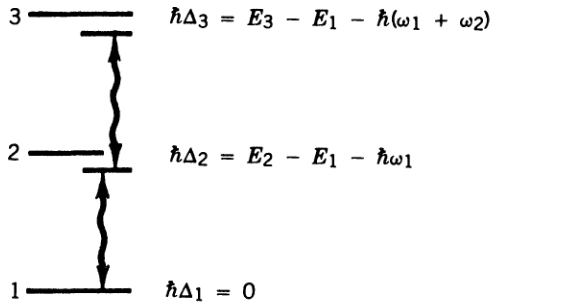
\includegraphics[width=\linewidth]{13-1-1a.png}
			\subcaption{ladder}
			\label{fig:13.1-1a}
			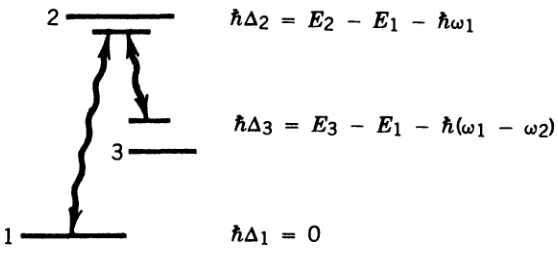
\includegraphics[width=\linewidth]{13-1-1b.png}
			\subcaption{lambda}
			\label{fig:13.1-1b}
			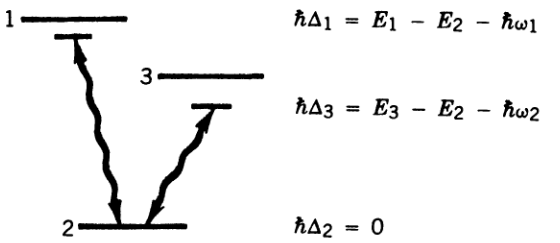
\includegraphics[width=\linewidth]{13-1-1c.png}
			\subcaption{vee}
			\label{fig:13.1-1c}
	\end{minipage}
	\caption{%Figure 13.1-1 
	Schematic diagram of three-state configurations
	%: \textit{(a)} ladder, \textit{(b)} lambda, \textit{(c)} vee.
	}
\end{wrapfigure}

First and simplest is the \textit{ladder configuration} in which the energies increases with index $ n, E_1 < E_2 < E_3 $, population initially resides in state 1, and loss occurs only from the uppermost state 3. Figure 13.1-1a % \ref should be inserted here.
illustrates this configuration. The convenient choice $ \Delta _1 = 0 $ \textit{is equivalent to \uline{setting the lowest energy $ E_1 $ to zero}}.

A second possibility, the \textit{lambda configuration}, occurs when the central energy of the sequence exceed either end-point energy, probability loss occurs again from the uppermost state, and initial population again resides in the lowest state. \ref{fig:13.1-1b} illustrates this configuration. Again the convenient choice $ \Delta _1 = 0 $ fixeds the energy zero point. The detuning $ \Delta _3 $ now involves differences between photon energies. More significantly (as we shall see in section $ \S $% \S is the "section" symbol.
13.7), loss occurs from the middle state of the sequence.
% Picture needed here.
\iffalse
\begin{figure}[h!]	%[h!] means 'precisely' 'here'
	\centering
	\begin{subfigure}[b]{0.33\linewidth}	% []: h (here) - same location; t (top) - top of page; b (bottom) - bottom of page; p (page) - on an extra page; ! (override) - will force the specified location
		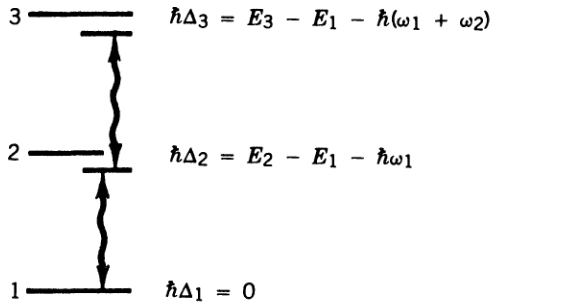
\includegraphics[width=\linewidth]{13-1-1a.png}
		\caption{ladder}
		\label{fig:13.1-1a}
	\end{subfigure}
	~ %add desired spacing between images, e. g. ~, \quad, \qquad, \hfill etc. 
      %(or a blank line to force the subfigure onto a new line)
	\begin{subfigure}[b]{0.33\linewidth}
		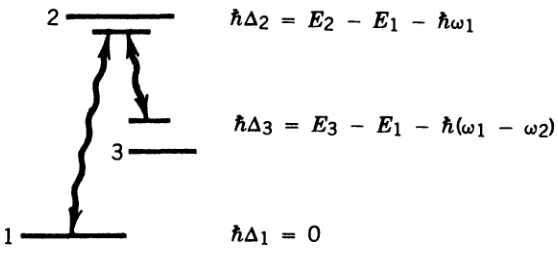
\includegraphics[width=\linewidth]{13-1-1b.png}
		\caption{lambda}
		\label{fig:13.1-1b}
	\end{subfigure}
	~
	\begin{subfigure}[b]{0.33\linewidth}
		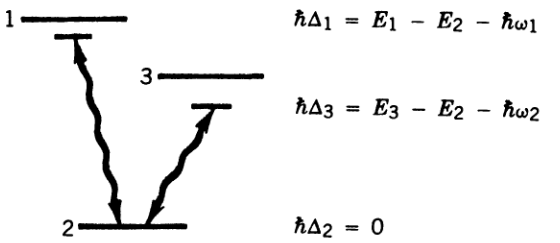
\includegraphics[width=\linewidth]{13-1-1c.png}
		\caption{vee}
		\label{fig:13.1-1c}
	\end{subfigure}
	\caption{%Figure 13.1-1 
	Schematic diagram of three-state configurations
	%: \textit{(a)} ladder, \textit{(b)} lambda, \textit{(c)} vee.
	}
\end{figure}
\fi

A third possibility the \textit{vee configuration}, occurs when the central state lies lowest in energy. \ref{fig:13.1-1c} %\textit{c}
illustrates this case. Here the convetional choice $ \Delta _2 = 0 $ fixes $ E_2 $ as the zero point of energy.

We shall see that each of these configurations gives rise to characteristic behavior of population flow. It should be apeciated that the discussion, being based upon the Schr\"odinger equation, refers to coherent excitation, not to the conventional incoherent rate-equation regime. For example, the diagram o the linkage pattern for the lambda system is that of the \textit{Raman scattering} process, in which a photon of one frequency is absorbed and a second frequency is reemitted. This two-photon process is usually observed under steady-state conditions, corresponding to a limit best treated by density matrix methods or rate equations.

\bigskip\noindent
\textbf{Summary of Rotating-Wave Phase Choices.} The various choices of phases are summarized by the following relationships:
% In the following, I tried to use a loop, but the equations seems too "irrugular".
\begin{comment}
	\newcommand{\RWPC}[1, 2]{
		& \dot{ \zeta _#1 } = 
		\begin{cases}
			\begin{matrix}
				\dot{ \zeta _#2 - \omega _1,\\
				\dot{ \zeta _#2 + \omega _1,
			\end{matrix}
		\end{cases}
		& \hbar \Delta _1 & \equiv E_1 - \hbar \dot{ \zeta _1 } = 
		\begin{cases}
			\begin{matrix}
				\hbar \Delta _2 + E_1 - E_2 + \hbar \omega_1, \qquad E_1 < E_2\\
				\hbar \Delta _2 + E_1 - E_2 - \hbar \omega_1, \qquad E_1 > E_2
			\end{matrix}
		\end{cases}\\}
	\DoWith\RWPC 123 \StopDoing
\end{comment}
% Beginning.
\begin{align*}
	& \dot{ \zeta _1 } = 
		\begin{cases}
		\begin{matrix}
			\dot{ \zeta _2 } - \omega _1,\\
			\dot{ \zeta _2 } + \omega _1,
		\end{matrix}
		\end{cases}		% \end{cases} produces an '{'.
	& \hbar \Delta _1 & \equiv E_1 - \hbar \dot{ \zeta _1 } = 
		\begin{cases}
		\begin{matrix}
			\hbar \Delta _2 + E_1 - E_2 + \hbar \omega_1, \qquad E_1  < E_2\\
			\hbar \Delta _2 + E_1 - E_2 - \hbar \omega_1, \qquad E_1  > E_2
		\end{matrix}
		\end{cases}\\
	& \dot{ \zeta _2 } = 
		\begin{cases}
		\begin{matrix}
			\dot{ \zeta _1 } - \omega _1,\\
			\dot{ \zeta _1 } + \omega _1,
		\end{matrix}
		\end{cases}
	& \hbar \Delta _2 & \equiv E_2 - \hbar \dot{ \zeta _2 } = 
		\begin{cases}
		\begin{matrix}
			\hbar \Delta _1 + E_2 - E_1 - \hbar \omega_1, \qquad E_1  < E_2\\
			\hbar \Delta _1 + E_2 - E_1 + \hbar \omega_1, \qquad E_1  > E_2
		\end{matrix}
		\end{cases}\\
	& \dot{ \zeta _3 } = 
		\begin{cases}
		\begin{matrix}
			\dot{ \zeta _2 } + \omega _2,\\
			\dot{ \zeta _2 } - \omega _2,
		\end{matrix}
		\end{cases}
	& \hbar \Delta _3 & \equiv E_3 - \hbar \dot{ \zeta _3 } = 
		\begin{cases}
		\begin{matrix}
			\hbar \Delta _2 + E_3 - E_2 - \hbar \omega_2, \qquad E_2  < E_3\\
			\hbar \Delta _2 + E_3 - E_2 - \hbar \omega_2, \qquad E_2  > E_3
		\end{matrix}
		\end{cases}
\end{align*}
\noindent
For the ladder system, with $ E_1 < E_2 < E_3 $ and the choice $ \Delta _1 = 0 $ the phases are
\begin{align*}
	& \dot{ \zeta _2 } = \dot{ \zeta _1 } + \omega _1,
	& \hbar \Delta _2 = E_2 - E_1 - \hbar \omega _1,\\
	& \dot{ \zeta _3 } = \dot{ \zeta _1 } + \omega _2,	% The original line of the .djvu must have unintentionally added a double '+\omega_2'.
	& \hbar \Delta _3 = E_3 - E_1 - \hbar \omega _2		% The original line of the .djvu must have unintentionally added '-\hbar\omega_1'.
\end{align*}
\noindent
For the lambda system, with $ E_1 < E_2, E_3 < E_2 $ and the choice $ \Delta _2 = 0 $ the phase are
\begin{align*}
	& \dot{ \zeta _1 } = \dot{ \zeta _2 } - \omega _1,
	& \hbar \Delta _1 = - ( E_2 - E_1 ) + \hbar \omega _1,\\
	& \dot{ \zeta _3 } = \dot{ \zeta _2 } - \omega _2,
	& \hbar \Delta _3 = - ( E_2 - E_3 ) + \hbar \omega _2.
\end{align*}
\noindent
For the vee system, with $ E_1 > E_2, \quad E_3 > E_2 $ and the choice $ \Delta _2 = 0 $ the phases are
\begin{align*}
	& \dot{ \zeta _1 } = \dot{ \zeta _2 } + \omega _1,
	& \hbar \Delta _1 = E_1 - E_2 - \hbar \omega _1,\\
	& \dot{ \zeta _3 } = \dot{ \zeta _2 } + \omega _2,
	& \hbar \Delta _3 = E_3 - E_2 - \hbar \omega _2.
\end{align*}

\bigskip\noindent
\textbf{Closed Loop Configuration.} I shall be discussing simple RWA systems involving two transitions amongst three states. It is also possible to consider three-state transitions combined with \textit{three} near-resonant excitation frequencies, in a linkage pattern that forms a closed loop. For a free atom (as distinguished from an atom embedded in a solid or other external field) at least one of the transitions of such a loop must be a forbidden transition, produced by magnetic dipole or electric quadrupole transition. This arrangement offers interesting possibilities for observation of the relative phase of the radiation, as discussed by Buckle et al. (1986).
		
\end{document}

